\documentclass[12pt]{article}
%\documentstyle[A4]{article}

\usepackage{listings}
%\usepackage{minted}
%\input amssym.def
%\newcommand{\Rr}{\Bbb R}
%\newcommand{\Qq}{\Bbb Q}
\usepackage{geometry}
%\usepackage{showframe} %This line can be used to clearly show the new margins
\newgeometry{vmargin={25mm}, hmargin={35mm,35mm}} 
\usepackage[autostyle]{csquotes}
\usepackage{hhline}
\usepackage{graphicx}
\usepackage{color}

\definecolor{dkgreen}{rgb}{0,0.6,0}
\definecolor{gray}{rgb}{0.5,0.5,0.5}
\definecolor{mauve}{rgb}{0.58,0,0.82}

\lstset{frame=tb,
	language=Python,
	aboveskip=3mm,
	belowskip=3mm,
	showstringspaces=false,
	columns=flexible,
	basicstyle={\ttfamily},
	numbers=none,
	numberstyle=\tiny\color{gray},
	keywordstyle=\color{blue},
	commentstyle=\color{dkgreen},
	stringstyle=\color{mauve},
	breaklines=true,
	breakatwhitespace=true,
	tabsize=4
}


\begin{document}
\title{Data Structures in Python}
\begin{center}
	\huge {Data Structures in Python}
\end{center}

\section{Sorting and Searching}
\subsection{Bubble sort ($\sim O(n^2)$)}
\begin{enumerate}
	\item Compare the first two elements of the list to check them which one is greater.
	\item For ascending ordering, place the larger value on the right.
	\item Do the same for second, third elements and so on till the whole list is completed. This is the first round.
	\item Execute steps (1), (2) and (3) for $n$ number of times where $n$ is the length of the list. (In second round you don't need to consider the last element. In third round no need to consider the last two elements and so on.)
\end{enumerate}
\begin{table}[h]
	\label{Bubble sort}
	\caption{\textbf{Bubble sort, Total round = length(list) - 1 =3}}
	\vspace{2mm}
	\centering
	\begin{tabular}{cccc}
		&{First round}  &{Second round}  &{Third round}   \\
		&\underline{7} \underline{2} 5 4  &\underline{2} \underline{5} 4 7&\underline{2} \underline{4} 5 7\\
		
		&2 \underline{7} \underline{5} 4&2 \underline{5} \underline{4} 7  &2 4 5 7   \\
		&2 5 \underline{7} \underline{4}  &2 4 5 7 &   \\
		&2 5 4 7  & &\\
		&Iteration num. = 3 &Iteration num. = 2 &Iteration num. = 1 
	\end{tabular}
\end{table}

\lstinputlisting[language=Python]{src/sort/bubblesort.py}
\textbf{Output:}
\begin{lstlisting}
Before sorting:
[54, 26, 93, 17, 77, 31, 44, 55, 20]
After bubble sort:
[17, 20, 26, 31, 44, 54, 55, 77, 93]
\end{lstlisting}

\subsection{Selection sort}
Number of comparisons $\sim O(n^2)$\\
Number of swaps $\sim O(n)$(?)
\begin{enumerate}
	\item The first element is compared with all other elements in the list one-by-one.
	\item If any element is found to be greater than any other element, then they are swapped.
	\item After the first iteration, the smallest number is placed at the first position. The same procedure is repeated for the second element and so on.
\end{enumerate}

\begin{table}[h]
	\label{Selection sort}
	\caption{\textbf{Selection sort, Total round = length(list) - 1 =3}}
	\vspace{2mm}
	\centering
	\begin{tabular}{cccc}
		&{First round}  &{Second round}  &{Third round}   \\
		&\underline{7} \underline{2} 5 4  &2 \underline{7} \underline{5} 4 &2 4 \underline{7} \underline{5}   \\
		&\underline{2} 7 \underline{5} 4 &2 \underline{5} 7 \underline{4}  &2 4 5 7   \\
		&\underline{2} 7 5 \underline{4}  &2 4 7 5 &   \\
		&2 7 5 4  & &\\
		&Iteration num. = 3 &Iteration num. = 2 &Iteration num. = 1 
	\end{tabular}
\end{table}

\lstinputlisting[language=Python]{src/sort/selectionsort.py}
\textbf{Output:}
\begin{lstlisting}
Before sorting:
[54, 26, 93, 17, 77, 31, 44, 55, 20]
After selection sort:
[17, 20, 26, 31, 44, 54, 55, 77, 93]
\end{lstlisting}
\subsection{Insertion sort ($\sim O(n^2)$)}

\begin{enumerate}
	\item The first iteration starts with comparing the first and second elements and ordering them accordingly.
	\item In second iteration, the third element is compared with the first and second elements and placed in a suitable position by shifting other elements.
	\item The procedure is repeated for all elements in the array.
\end{enumerate}

\begin{figure}[h]
	\centering
	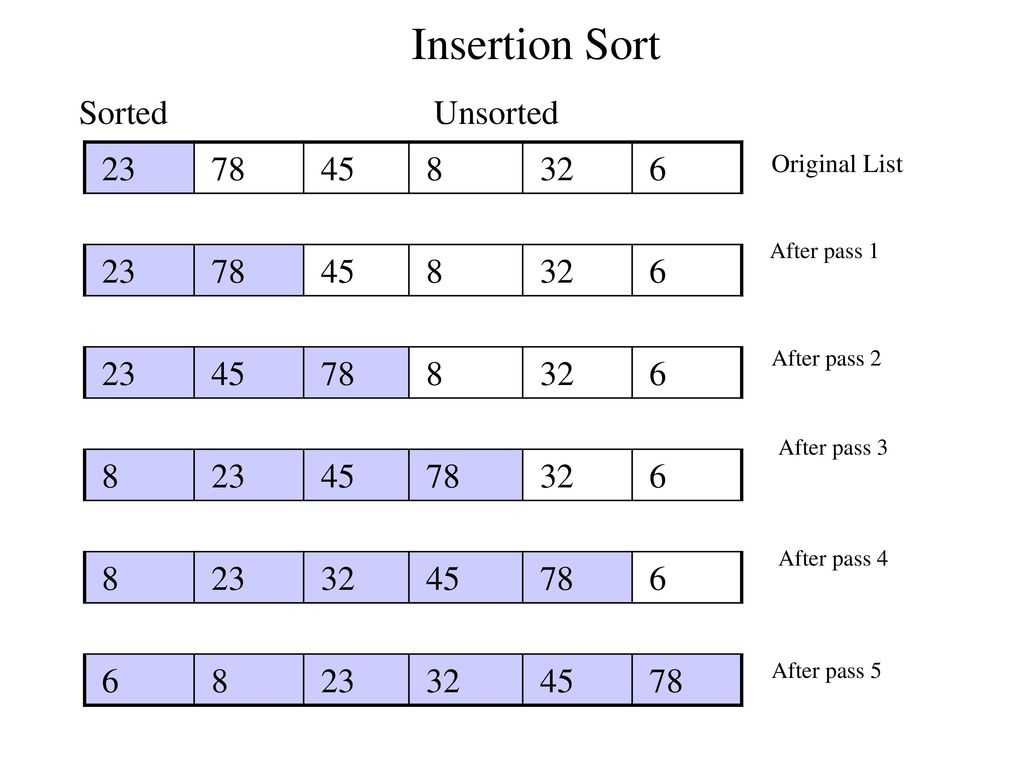
\includegraphics[scale=1.2]{src/sort/pic/picinsertion.jpg}
\end{figure}

\lstinputlisting[language=Python]{src/sort/insertionsort.py}
\textbf{Output:}
\begin{lstlisting}
Before sorting:
[54, 26, 93, 17, 77, 31, 44, 55, 20]
After insertion sort:
[17, 20, 26, 31, 44, 54, 55, 77, 93]
\end{lstlisting}

\newpage
\section{Stack}
Stacks are the data structures in which the items to be inserted or removed follow the \textbf{Last-in-First-out} (LIFO) principle. The insertion or deletion of items takes place one end of the stack known as the \textbf{top} of the stack. 

When an item is added into a stack, the operation is called \textbf{push} and when an item is removed from the stack, the operation is called \textbf{pop}.

Most microprocessors use a stack-based architecture. When a method (sub-routine) is called, its return address is pushed onto a stack and when it returns, the address is popped off.\\

\textbf{Applications of stack:}

\begin{itemize}
	\item Reversing a word: You push a word onto a stack letter-by-letter and then pop letters from the stack.
	\item Doing `undo' mechanism in text editors. This is accomplished by keeping all text changes in a stack.
	\item Compiler's syntax check for matching parentheses is acomplished by using stack.
\end{itemize}


\lstinputlisting[language=Python]{src/Stack.py}
\textbf{Output:}
\begin{lstlisting}
| 4 |
-----
| 31 |
------
| A |
-----
| 1 |
-----
Popped item = 4
| 31 |
------
| A |
-----
| 1 |
-----
Reverse of 'Hello' is olleH
Binary of '242' is 11110010
[a+b][c+d]: True
[a+b][c+}d]: False
\end{lstlisting}

\newpage
\section{Queue}
Queue is an abstract data type or a linear data structure in which the addition of items takes place from one end called the \textbf{REAR}(also called \textbf{tail}), and the removal of existing items takes place from the other end called as \textbf{FRONT}(also called \textbf{head}).

This makes queue as \textbf{FIFO}(First in First Out) data structure, which means that element inserted first will be removed first.
The process to add an element into queue is called \textbf{Enqueue} and the process of removal of an element from queue is called \textbf{Dequeue}.\\

\vspace{3mm}
\textbf{Applications of Queue:}
\begin{itemize}
	\item Serving requests on a single shared resource, like a printer, CPU task scheduling etc.
	\item Handling of interrupts in real-time systems. The interrupts are handled in the same order as they arrive i.e First come first served.
	\item Phone answering system: The person who calls first gets a response first from the phone answering system.
\end{itemize}

\lstinputlisting[language=Python]{src/queue.py}
\textbf{Output:}
\begin{lstlisting}
| 3 | dog | hello |
Removed item = hello
| 3 | dog |
| 61 | 3 | dog |
Queue size = 3
\end{lstlisting}
\newpage

\section{Deque}
Deque or double ended queue is a generalized version of queue data structure that allows insert and delete at both ends.

What makes a deque different is the unrestrictive nature of adding and removing items. New items can be added at either the front or the rear. Likewise, existing items can be removed from either end. In a sense, this hybrid linear structure provides all the capabilities of stacks and queues in a single data structure.\\

\lstinputlisting[language=Python]{src/deque.py}
\textbf{Output:}
\begin{lstlisting}
| 4 |
| dog | 4 |
| dog | 4 | cat |
| dog | 4 | cat | 45 |
Deque size = 4
| dog | 4 | cat | 45 |
Removed item from rear = dog
| 4 | cat | 45 |
Removed item from front = 45
| 4 | cat |
\end{lstlisting}


\subsection{Palindrome Checker}

An interesting problem that can be easily solved using the deque data structure is the classic palindrome problem. A palindrome is a string that reads the same forward and backward, for example, radar, madam etc.\\

\lstinputlisting[language=Python]{src/palindrome.py}
\textbf{Output:}
\begin{lstlisting}
False
True
\end{lstlisting}
\subsection{Python collection.deque module}
Deque can be implemented in python using the module "collections".\\
 
\lstinputlisting[language=Python]{src/deque2.py}
\textbf{Output:}
\begin{lstlisting}
deque([1, 2, 3])
Insert 4 at right: deque([1, 2, 3, 4])
Insert 6 at left: deque([6, 1, 2, 3, 4])
Delete from right: deque([6, 1, 2, 3])
Delete from right: deque([1, 2, 3])
~~~~~~~~~~~~~~~~~~~~~~~~~~~~~~~~~~~~~~~~
deque([1, 2, 3, 3, 4, 2, 4])
Number 4 first occurs at: 4
After inserting 3 at 5th position: 
deque([1, 2, 3, 3, 3, 4, 2, 4])
Count of 3 : 3
After deleting first occurrence of 3: 
deque([1, 2, 3, 3, 4, 2, 4])
~~~~~~~~~~~~~~~~~~~~~~~~~~~~~~~~~~~~~~~~
deque([1, 2, 3])
The deque after extending deque at end: 
deque([1, 2, 3, 4, 5, 6])
The deque after extending deque at beginning: 
deque([9, 8, 7, 1, 2, 3, 4, 5, 6])
The deque after rotating deque: 
deque([1, 2, 3, 4, 5, 6, 9, 8, 7])
\end{lstlisting}


\newpage
\section{Linked List}

A linked list is a linear collection of data elements in which the linear ordering is maintained by each element pointing to the next (not by physical placements in memory). It is a data structure consisting of a group of nodes which together form a sequence. Each node is composed of two parts: \textbf{data} and a \textbf{reference} (link) to the next node in the sequence.\\

\textbf{Advantages:}
\begin{enumerate}
	\item Unlike list (array), they are dynamic in nature which allocates memory whenever required.
	\item This structure allows efficient insertion and removal of elements.
	\item Stacks and queues can easily be implemented.
	\item Linked list reduces the access time.
\end{enumerate}

\textbf{Disadvantages:}
\begin{enumerate}
	\item The memory is wasted as the reference requires extra memory for storage.
	\item No element can be accessed randomly.
	\item Reverse traversing is difficult.
\end{enumerate}


\lstinputlisting[language=Python]{src/Linkedlist.py}
\textbf{Output:}
\begin{lstlisting}
[A] ---> [B] ---> [C] ---> None
[A] ---> [5] ---> [B] ---> [D] ---> [C] ---> None
[A] ---> [5] ---> [D] ---> [C] ---> None
[C] ---> [D] ---> [5] ---> [A] ---> None
Search value index = 3
[C] ---> [D] ---> [5] ---> [A] ---> None
\end{lstlisting}

\newpage
\section{Binary Search Tree}
\lstinputlisting[language=Python]{src/BinaryTree/BinarySearchTree.py}
\textbf{Output:}
\begin{lstlisting}
Could not find the node with data = 75
The data in the parent node is 5
Inorder traversing -->
1 5 10 13 14
Preorder traversing -->
10 5 1 13 14
Preorder traversing -->
1 5 14 13 10
Removing node with two children...
Removing Node with single left child...
\end{lstlisting}

\section{Heap}
Heap data structure is a \textit{complete binary tree} that satisfies the\textit{ heap property}. It is also called as a binary heap. 
A \textit{complete binary} tree is a special binary tree in which satisfies the following conditions -
\begin{itemize}
	\item Each level is completely filled before another level is added.
	\item The bottom tier is filled in from left to right.
\end{itemize}
\textit{Heap Property} is the property of a node which satisfies the following conditions -
\begin{itemize}
	\item Max heap: Data(key) of each node is always greater than its child node(s).
	\item Min heap: Data(key) of each node is always smaller than its child node(s).
\end{itemize}
Another interesting property of a complete tree is that we can represent it using a single list. Because the tree is complete, for a node at index $p$ in the parent,
\begin{itemize}
	\item Its parent is at $\frac{p-1}{2}$ (integer division).
	\item Its left child is at $2p+1$.
	\item Its right child is at $2p+2$.
\end{itemize}
\lstinputlisting[language=Python]{src/Heap/Heap.py}
\textbf{Output:}
\begin{lstlisting}
[82, 70, 53, 63, 27, 43, 37, 10, 51]
[70, 63, 53, 51, 27, 43, 37, 10]
\end{lstlisting}
\end{document}